\documentclass[letterpaper]{article}
\usepackage[utf8]{inputenc}
\usepackage{url}
\usepackage{aaai}
\usepackage{times}
\usepackage{helvet}
\usepackage{courier}
\usepackage{amsmath}
\usepackage{amssymb}
\usepackage{graphicx}

\begin{filecontents}{references_final.bib}
@article{wang2020fuelnet,
    title = "FuelNet: A precise fuel consumption prediction model using long short-term memory deep network for eco-driving",
    author = "Wang, Guanqun and Zhang, Licheng and Xu, Zhigang and Hina, Syeda Mahwish and Sun, Pengpeng and Min, Haigen and Wei, Tao and Qu, Xiaobo",
    year = "2020"
}

@article{abukhalil2020fuel,
    title = "Fuel Consumption Using OBD-II and Support Vector Machine Model",
    author = "Abukhalil, Tamer and AlMahafzah, Harbi and Alksasbeh, Malek and Alqaralleh, Bassam AY",
    journal = "Journal of Robotics",
    volume = "2020",
    number = "1",
    pages = "9450178",
    year = "2020",
    publisher = "Wiley Online Library"
}

@article{yen_combining_2021,
    author = "Yen, Meng-Hua and Tian, Shang-Lin and Lin, Yan-Ting and Yang, Cheng-Wei and Chen, Chi-Chun",
    title = "Combining a Universal OBD-II Module with Deep Learning to Develop an Eco-Driving Analysis System",
    journal = "Applied Sciences",
    volume = "11",
    year = "2021",
    number = "4481",
    url = "https://www.mdpi.com/2076-3417/11/10/4481",
    issn = "2076-3417"
}

@article{rykala2023modeling,
    title = "Modeling vehicle fuel consumption using a low-cost OBD-II interface",
    author = "Ryka{\l}a, Magdalena and Grzelak, Ma{\l}gorzata and Ryka{\l}a, {\L}ukasz and Voicu, Daniela and Stoica, Ramona-Monica",
    journal = "Energies",
    volume = "16",
    number = "21",
    pages = "7266",
    year = "2023",
    publisher = "MDPI"
}

@article{filla2025using,
    title = "Using Weather Data for Improved Analysis of Vehicle Energy Efficiency",
    author = "Filla, Reno",
    journal = "Data",
    volume = "10",
    number = "3",
    pages = "31",
    year = "2025",
    publisher = "MDPI"
}

@article{Manjunath2024,
    author = "Manjunath, T.K. and Ashok Kumar, P.S.",
    title = "Fuel Prediction Model for Driving Patterns Using Machine Learning Techniques",
    journal = "Journal of Computer Science",
    volume = "20",
    number = "3",
    pages = "291--302",
    year = "2024",
    doi = "10.3844/jcssp.2024.291.302",
    publisher = "Science Publications",
    url = "https://thescipub.com/pdf/jcssp.2024.291.302"
}

@article{zhang2023novel,
    title = "Novel Neural-Network-Based Fuel Consumption Prediction Models Considering Vehicular Jerk",
    author = "Zhang, Licheng and Ya, Jingtian and Xu, Zhigang and Easa, Said and Peng, Kun and Xing, Yuchen and Yang, Ran",
    journal = "Electronics",
    volume = "12",
    number = "17",
    pages = "3638",
    year = "2023",
    publisher = "MDPI"
}

@article{topic2022neural,
    title = "Neural network-based prediction of vehicle fuel consumption based on driving cycle data",
    author = "Topi{\'c}, Jakov and {\v{S}}kugor, Branimir and Deur, Jo{\v{s}}ko",
    journal = "Sustainability",
    volume = "14",
    number = "2",
    pages = "744",
    year = "2022",
    publisher = "Multidisciplinary Digital Publishing Institute"
}

@article{abediasl2024real,
    title = "Real-time vehicular fuel consumption estimation using machine learning and on-board diagnostics data",
    author = "Abediasl, Hamidreza and Ansari, Amir and Hosseini, Vahid and Koch, Charles Robert and Shahbakhti, Mahdi",
    journal = "Proceedings of the Institution of Mechanical Engineers, Part D: Journal of Automobile Engineering",
    volume = "238",
    number = "12",
    pages = "3779--3793",
    year = "2024",
    publisher = "SAGE Publications Sage UK: London, England"
}

@article{yang2022predicting,
    title = "Predicting gasoline vehicle fuel consumption in energy and environmental impact based on machine learning and multidimensional big data",
    author = "Yang, Yushan and Gong, Nuoya and Xie, Keying and Liu, Qingfei",
    journal = "Energies",
    volume = "15",
    number = "5",
    pages = "1602",
    year = "2022",
    publisher = "MDPI"
}

@article{al2007experimental,
    title = "Experimental investigation of factors affecting vehicle fuel consumption",
    author = "Al-Momani, Walid M and Badran, Omar",
    journal = "International Journal of Mechanical and Materials Engineering",
    volume = "2",
    number = "2",
    pages = "180--188",
    year = "2007",
    publisher = "University of Malaya"
}

@article{hegde2021real,
    title="Real-world driving features for identifying intelligent driver model parameters",
    author="Hegde, Bharatkumar and O'Keefe, Michael and Muldoon, Steven and Gonder, Jeffrey and Chang, Chen-Fang",
    year="2021",
    institution="National Renewable Energy Lab.(NREL), Golden, CO (United States)"
}

@article{Bandgar2024,
  author = "Aaditya Bandgar and Pratik Barge and Abhishek Bhamare and Somesh Bhamre and Giridhar Bhande and Ganesh Korwar",
  title = "Design of Variable Valve Timing and Electronic Control for Honda R18A",
  journal = "International Journal for Research in Applied Science and Engineering Technology (IJRASET)",
  volume = "12",
  number = "V",
  pages = "507--512",
  year = "2024"
}

@misc{nrel_routee,
    author = "National Renewable Energy Laboratory NREL",
    organization = "National Renewable Energy Laboratory",
    year = "2017",
    title = "Route{E}: Route {E}nergy {P}rediction {M}odel",
    url = "https://www.nrel.gov/transportation/route-energy-prediction-model.html"
}

@misc{google_2023_environmental_report,
    author = "Google",
    organization = "Google Inc.",
    year = "2023",
    title = "Google 2023 {E}nvironmental {R}eport",
    url = "https://www.gstatic.com/gumdrop/sustainability/google-2023-environmental-report.pdf"
}

\end{filecontents}

\frenchspacing
\setlength{\pdfpagewidth}{8.5in}
\setlength{\pdfpageheight}{11in}
\pdfinfo{
/Title (Temperature-Dependent Estimation of Vehicle Fuel Economy: Experimental Methodology)
/Author (Sindu Chitraju, Samuel Howard, Seif Ilkbarieh, Om Solanki, Andrew Wheeler)}
\setcounter{secnumdepth}{0}  

\begin{document}

% The file aaai.sty is the style file for AAAI Press 
% proceedings, working notes, and technical reports.

% Remove the copyright from the footer
\nocopyright

\title{Temperature-Dependent Estimation of Vehicle Fuel Economy}
\author{Sindu Chitraju, Samuel Howard, Seif Ilkbarieh, Om Solanki, Andrew Wheeler\\
Tennessee Technological University
}

\maketitle

\begin{abstract}
\begin{quote}
    This project proposes to investigate the application of Recurrent Neural Networks (RNNs) to predict vehicle fuel economy using accessible on-board diagnostics II (OBD-II) data. 
    Leveraging the temporal dependencies inherent in driving patterns, we aim to develop a model that accurately predicts fuel consumption based on a sequence of sensor readings for a single vehicle.
    This approach offers a personalized and adaptable alternative to generalized fuel economy estimates, further contextualized with external climate data for even more accurate estimates.
    % We will explore various RNN architectures and evaluate their performance using real-world driving data collected from a personal vehicle. 
    This has the potential to contribute to fuel efficiency optimization, personalized driver feedback systems, and more accurate route planning tools. 
\end{quote}
\end{abstract}

\section{Introduction}

\noindent Fuel economy is a critical concern with economic and environmental implications. 
While standardized tests provide a general idea of the performance of a vehicle, 
real-world fuel consumption varies significantly based on driving style, traffic conditions, and other factors.
This project addresses the need for route-specific, weather-dependent fuel economy prediction by leveraging the power of RNNs to model the temporal relationships within driving data.
We hypothesize that RNNs can learn the intricate dependencies between many of the variables that contribute to fuel economy including temperature, a metric that is not often accounted for.
% The result of this work could empower drivers to optimize their driving habits whilst vehicle manufacturers could optimize aspects of vehicle drivetrains to account for environmental conditions.

\section{Related Work}

% This project builds upon existing research in fuel economy modeling and route planning. 
% The NREL's REPM, which powers fuel efficient routing in Google Maps, 
% demonstrates the value of accurate fuel consumption prediction, 
% preventing more than 1.2 million metric tons of carbon emissions \cite{google_2023_environmental_report}.
% While REPM uses aggregated and generalized data from a few vehicles, 
% our approach leverages the richness and breadth of vehicle sensor data from a single vehicle for better accuracy \cite{nrel_routee}.

%%%%%%%%%%%%%%%%%%%%%%%%%%%%%%%%%%%%%%%%%%%%%%%%%%%%%%%%%%%%%%%%%%%%%%%%%%%

% Drew
\subsection*{Experimental Investigation of Factors Affecting Vehicle Fuel Consumption}

Previous work has already been completed that evaluates a number of factors that
can influence the fuel efficiency of vehicles. The work of \cite{al2007experimental}
tests a number of parameters, including altitude, vehicle speed, and
tire pressure, to name a few. The authors evaluated a number of vehicle makes
and models, with the model years used spanning nearly a decade and a half. 

To measure fuel consumption, a flow rate sensor was integrated into the fuel line
between the fuel tank and fuel pump of the tested vehicles. Because the sensor
is part of the supplying fuel line, high-accuracy measurements can be obtained
without having to make significant modifications to more complicated components,
such as the engine. 

While this work takes into account a large number of
parameters and their impact on fuel economy, the cars utilized in the experiment
are not accurate reflections of modern internal combustion engines. Additionally, the
authors had to make modifications to the car's fuel line to integrate the sensor.
While this provides very accurate measurements, it is beyond what can be
considered an easily accessible method of measurement.

\subsection*{Predicting Gasoline Vehicle Fuel Consumption in Energy and Environmental 
Impact Based on Machine Learning and Multidimensional Big Data}

The work of \cite{yang2022predicting} evaluates the real-world fuel economy performance of 
vehicles, comparing this to the estimated values provided by car manufacturers. 
The authors then utilized a number of machine learning algorithms in an attempt to 
create accurate predictions of fuel consumption based on a number of criteria.

Real-world fuel economy data was collected via the BearOil app, containing reported fuel 
efficiency from the app's users. Additionally, behavioral data of users' driving habits was 
gathered using a basic twenty-question survey. The collected data was cleaned and five models 
were trained over it: a linear regression, Naive Bayes, neural network, random forest, 
and Light Gradient-Boosting Machine (LightGBM). 

While \cite{yang2022predicting} take a very large-scale approach, having nearly one million 
records to train models over, their scope is quite large and attempts to predict fuel 
consumption using a fair number of qualitative data points, such as a driver's ability. 
Additionally, the focus of their  work is on how multiple models perform in the context of 
each other, as opposed to how accurate a single model can be.

\subsection*{Experimental Investigation of the Impact of Jerk on Vehicle Fuel
Consumption Prediction}

The work of \cite{zhang2023novel} evaluates the effects of vehicle jerk, where large
changes in speed occur over a very short period of time, on fuel economy. 

The authors then attempt to use data preprocessing and machine learning models to
make accurate predictions, regardless of the presence of jerk in the data. The
authors utilized a system that integrated a global positioning system (GPS) and
on-board diagnostic (OBD) interface, allowing them to gather high-accuracy,
high-precision positional data and real-time statistics on the state of the
vehicle. 

Where this work differs is that it utilizes multiple machine learning models and
evaluates their performance in the context of each other. Our proposal focuses
on a single model and the extent to which it can accurately predict fuel
consumption.

% Samuel
\subsection*{Modeling Vehicle Fuel Consumption Using a Low-Cost OBD-II Interface}

\cite{rykala2023modeling} developed an innovative approach to modeling vehicle fuel
consumption by leveraging data collected using a low-cost OBD2 adapter alongside
onboard phone sensors. Their study aimed to explore and compare various
predictive modeling techniques to identify the most effective method, using
parameters such as GPS coordinates, driving speed, and additional signals
processed through the vehicle's diagnostic system and phone sensors. With this
data, they implemented and tested three distinct types of models: a multivariate
regression model, decision trees, and a set of 750 multilayer perceptron (MLP)
models. Among these, the MLP models demonstrated the greatest accuracy, making
them the most reliable choice for forecasting fuel consumption under diverse
driving conditions. 

They captured data from a test drive of approximately 320
kilometers (199 miles) on a selected route. Data collected includes engine speed
(RPM), vehicle speed, gear, acceleration, engine load, and road slope based on a
moving average. Of these, the most important variables were gear, speed, and
engine load. Information for the gear was determined with a linear regression of
vehicle speed and engine speed.

\subsection*{Combining a Universal OBD-II Module with Deep Learning to Develop
an Eco-Driving Analysis System}

Greater accuracy can still be gained using larger networks. \cite{yen_combining_2021} 
explore utilizing Elman Recurrent Neural Network (RNN) and Feed-Forward Backpropagation
(FFB) models to predict fuel consumption with the goal of progressing
energy-saving and safe-driving developments. To this end, they collected data
from several vehicles to feed these networks. Their key contribution is their
models, combined with a graphical user interface for actionable driver feedback.
This includes engine speed, vehicle speed, and other driving behavior metrics.

For their data, they used three vehicles driven on a mix of relatively flat and
mountainous roads common in western Taiwan. Each of the vehicles was driven
along the same 209-kilometer (130-mile) route. This data was cleaned and
normalized before it was used for training the models. For comparison, they
calculated the instantaneous fuel consumption mathematically.

% Saif

\subsection*{Fuel Consumption Using OBD-II and Support Vector Machine Model}

The authors in \cite{abukhalil2020fuel} introduce a Machine Learning (ML)-based
model to estimate real-time fuel consumption by collecting data from an OBD-II
scanner. The authors’ model combines a Support Vector Machine (SVM) algorithm
with Lagrange interpolation to analyze the relationship between engines
parameters and fuel consumption. The engine parameters include Revolutions Per
Minute (RPM) and Throttle Position Sensor (TPS). To validate their model, the
authors use Mass Air Flow (MAF)-based calculations. The authors conduct their
experiments on a fixed 66 kilometer highway route using three gasoline-powered
vehicles that have different engine displacements and horsepowers. The author’s
model was able to achieve a Root-Mean-Square Error (RMSE) score of 2.4364,
proving its potential in predicting fuel consumption. 

The data employed in this
work was collected from three test-vehicles, namely a 2017 Ford Fusion, 2016
Toyota Camry, as well as a 2006 Mercedes-Benz E280. A CDP Autocom OBD-II scanner
was connected to every car, and the data points were collected during a
40-minute drive along a steep 66 kilometer route in different areas in Jordan.
The authors were able to collect 160 sample points during the drive, and the
data points include time-series readings of engine RPM, vehicle speed, throttle
position, and corresponding fuel consumption rates. The data points were used to
build polynomial regression models and evaluate the prediction accuracy of fuel
consumption against standard manufacturer values and traditional estimation
formulas. Overall, the authors' model was able to show the influence that engine
size has on fuel consumption in real-world scenarios.

\subsection*{Using Weather Data for Improved Analysis of Vehicle Energy
Efficiency}

The work of \cite{filla2025using} examines how weather conditions impact vehicle energy
efficiency, particularly for battery electric vehicles (BEVs). While previous
research has explored energy efficiency models, this paper stands out by using
national meteorological data to refine estimates of energy loss and improve
predictions of vehicle performance. 

The data sources include Swedish
institutions, as well as international ones like MET Norway and Deutscher
Wetterdienst. The study combines GNSS-based vehicle logs with weather data,
using two efficient algorithms to match weather conditions to the vehicle's
location and time. Filla compares in-vehicle sensor data to both weather station
data and interpolated weather data to assess accuracy and relevance. 

Although the research focuses on EVs and doesn't cover gasoline vehicles, it offers
valuable insight into how weather data can be used to better predict energy
efficiency. This approach could guide our project to answer the questions.

% Om
\subsection*{Fuel Prediction Model for Driving Patterns Using Machine Learning
Techniques}

\cite{Manjunath2024} explore a machine learning-based approach to predict and improve
fuel consumption by analyzing how people drive. They used linear regression and
support vector regression to estimate fuel efficiency, with the goal of
encouraging eco-friendly driving and cutting down on greenhouse gas emissions.

To gather real-world data, they used an ELM 327 OBD-II tool connected to a
laptop, which recorded 13 different sensor readings from the car. The data was
cleaned, normalized, and fine-tuned to highlight the most relevant driving
factors before being used to train the models. 

They evaluated the models using
standard metrics like R-squared, MSE, MAE, and RMSE, and found that linear
regression performed especially well. This paper lines up closely with what
we're working on, especially since they also used an OBD-II tool for data
collection. It offers some solid ideas for how we might approach fuel efficiency
prediction. That said, they only tried two machine learning techniques---so
there may be room for us to explore and find an even better-performing model.

% Seif
\subsection*{FuelNet: A precise fuel consumption prediction model using long
short-term memory deep network for eco-driving}

The authors in \cite{wang2020fuelnet} introduced FuelNet, which is a Long
Short-Term Memory (LSTM)-based Deep Learning (DL) model designed to predict fuel
consumption in different driving scenarios. The authors argue that there is
limited research being done on physics-based and shallow learning model. As a
result, they leverage the long-term dependency capabilities of LSTM networks to
work on their time-series vehicle data. The architecture of FuelNet is composed
of three layers and has been optimized for input efficiency, allowing it to
achieve a high Coefficient of Determination (R2) prediction score of 90.1\% while
using limited computational resources. FuelNet outperformed models like VSP,
VT-Micro, GRNN, RNN, and GRU in terms of error rates and generalizability. 

As for the data employed in this work, the authors used time-series data collected
from vehicles to train and test FuelNet. Their data specifically captures five
features, namely vehicle speed, acceleration, GPS coordinates, as well as fuel
consumption. The data they used was captured over a fixed distance of 300 meters,
and across various driving states such as high-speed, optimal-speed, and
stop-and-go conditions. Their data also supports speed ranges between 10 and 80
kilometers per hour, allowing FuelNet to learn various fuel consumption patterns.
To collect the ideal set of features for the prediction process, the authors
conducted several experiments using different input combinations. The authors
determined that speed and acceleration as input allowed FuelNet to achieve its
highest accuracy. Additionally, the data used included real-world scenarios,
such as data from Shaanxi Motor Trucks. This allowed the authors to validate the
anomaly detection capabilities of FuelNet, which helps in identifying issues
such as fuel leaks effectively. Overall, FuelNet was able to prove its
practicality in detecting abnormal fuel consumption trends, thereby enhancing
driving efficiency.

\subsection*{Real-time vehicular fuel consumption estimation using machine
learning and on-board diagnostics data}

\cite{abediasl2024real} explore machine learning for real-time fuel consumption estimation
using onboard diagnostics (OBD) data from fleet vehicles. Traditional methods,
like ECU-based estimates, can be inaccurate or expensive, so they tested four
models: Random Forest (RF), Artificial Neural Networks (ANN), Support Vector
Machines (SVM), and k-Nearest Neighbors (KNN). RF and ANN performed the best, so
they focused on comparing these two. 

They collected OBD data from different
vehicle types (sedans, SUVs, pickup trucks) with various powertrains, including
hybrids, and included cold-start conditions to capture fuel consumption during
engine warm-up. The models were trained and tested using a 70-30 data split with
five-fold cross-validation to improve reliability. 

RF handled different driving
conditions better, especially in urban areas, because it avoided overfitting and
worked well with diverse data. ANN required data normalization but still had
higher errors, particularly in stop-and-go traffic. Both models outperformed
traditional ECU-based methods, proving that machine learning is a strong option
for fuel prediction. This study is relevant to our work because it also focuses
on OBD data and machine learning for fuel estimation. Their findings suggest RF
is a strong choice, but there's room to explore additional models or
optimizations to improve accuracy further. Future research could test different
driving conditions, incorporate more OBD parameters, or use hybrid models that
combine multiple approaches for even better results.

\subsection{Neural Network-Based Prediction of Vehicle Fuel Consumption Based on
Driving Cycle Data}

\cite{topic2022neural} used neural networks to predict vehicle fuel consumption based on
driving cycle data, including speed, acceleration, and road slope. Traditional
models, like linear regression, don't always capture these factors well, so they
developed a two-stage neural network model---one part predicts driving patterns,
and the other estimates fuel use. 

They trained and tested their model using six months of GPS and CAN bus data from city buses 
in Dubrovnik. The data was broken down into smaller driving cycles, and synthetic cycles 
were generated to improve prediction accuracy. Their results showed that neural networks 
outperformed traditional models in both accuracy and speed. 

A key finding was that road slope had a big impact on fuel consumption, making it an 
important factor to include. The model also showed potential for real-world applications 
like optimizing vehicle routes, validating driving cycle data, and even estimating battery
charge levels for electric vehicles. The study suggests that using advanced machine learning 
techniques can lead to better fuel efficiency insights, helping both policymakers and 
transportation companies make informed decisions. Additionally, their approach could be 
adapted for different vehicle types or extended to analyze environmental impacts related 
to fuel consumption.

%%%%%%%%%%%%%%%%%%%%%%%%%%%%%%%%%%%%%%%%%%%%%%%%%%%%%%%%%%%%%%%%%%%%%%%%%%%

\section*{Our Dataset}
This project studies the predictive performance of recurrent neural network 
models on vehicle telemetry data, with a particular focus on how external 
and derived features works such as weather conditions, smoothed signals, 
and road grade that are influence by the accuracy of fuel consumption 
estimation. To conduct this study, we created multiple variants of the 
dataset and trained models under controlled conditions to remove the 
effects of each feature group.

The raw data used in this project was collected through the Torque mobile 
application, which logs real-time vehicle sensor data. These logs were 
cleaned and processed to ensure consistency and usability for machine 
learning. But only essential features such as engine RPM, throttle 
position, fuel usage, speed, altitude, and positional coordinates were 
retained. Duplicate entries were removed, and invalid/corrupted values, 
particularly those found in the fuel usage field, were filtered out. 
Instant fuel consumption values were pulled by computing the difference 
between successive readings of the cumulative trip fuel usage. The 
terrain slope, referred to as grade, was calculated using changes in 
altitude and vehicle speed to reflect shifts in road incline. 
Historical weather data was integrated into the dataset using the 
Open-Meteo API, with temperature values mapped to each GPS coordinate 
and timestamp. In some versions of the dataset, a moving average filter 
was applied to smooth the time-series data and reduce the impact of sensor 
noise.

\section*{Our Dataset Attributes}

\subsection*{Vehicular Factors}

From our dataset, a few key metrics emerged concerning fuel consumption. 
The most obvious correlation is speed. As speed increases, drag increases 
with the square of velocity according to the equation: 
\[
    \displaystyle F_{\mathrm {D} }\,=\,{\tfrac {1}{2}}\,\rho \,v^{2}\,C_{\mathrm {D} }\,A
\] 

This, along with the peak efficiency of internal combustion engines (ICE), 
leads to a peak fuel economy that is generally found between 45 and 55 MPH. 
In our data, this peak is at roughly 50 MPH, as shown in Figure \ref{fig:mpgspeed}. 
As seen in Figure \ref{fig:histmpgspeed}, the amount of data we have drops off sharply 
past 60 MPH, 5 MPH above the common speed limit of highways in the United 
States.

% speed_vs_mpg.png figure
\begin{figure}[htbp]
    \centering
    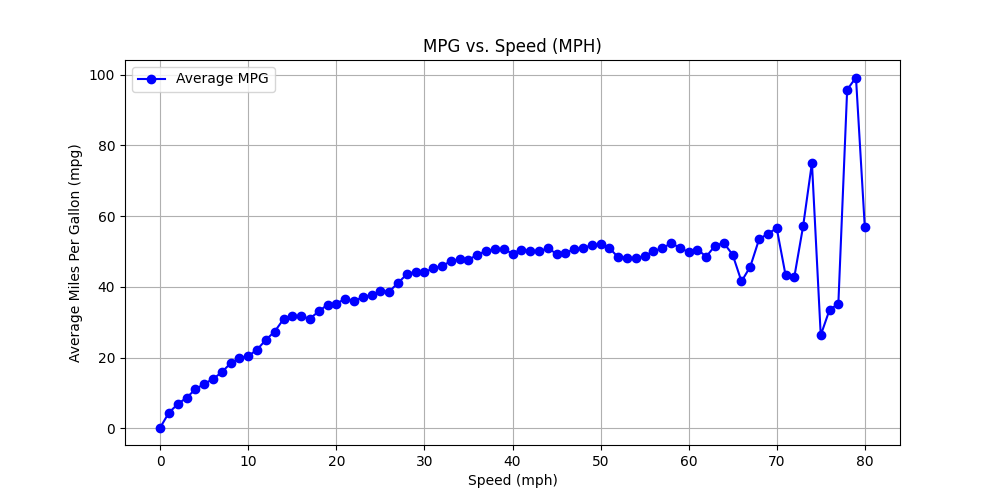
\includegraphics[width=0.4\textwidth]{figures/speed_vs_mpg.png}
    \caption{Plot of speed vs MPG}
    \label{fig:mpgspeed}
\end{figure}

% histogram_speedobdmph.png figure
\begin{figure}[htbp]
    \centering
    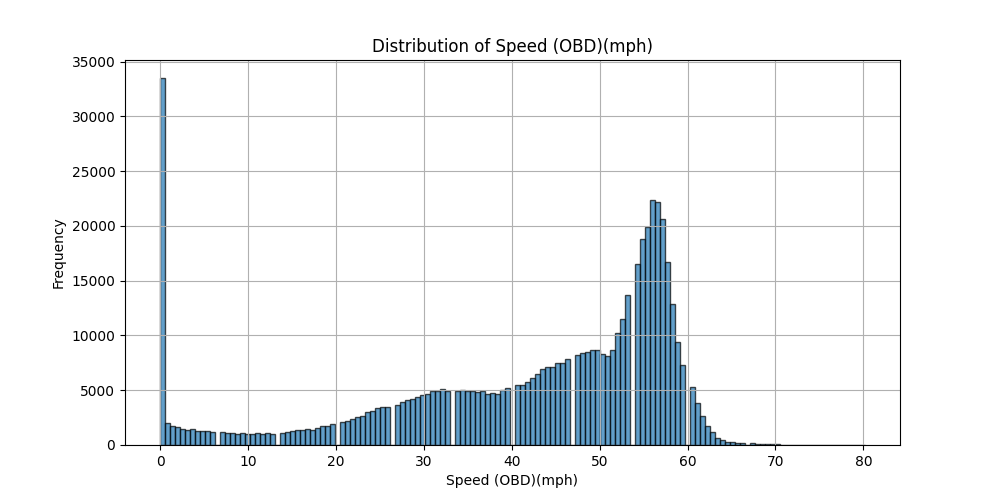
\includegraphics[width=0.4\textwidth]{figures/histogram_speedobdmph.png}
    \caption{Histogram of speed}
    \label{fig:histmpgspeed}
\end{figure}

Next on the list is temperature. The primary effect this has on fuel 
consumption is the density of the air entering the engine. Warmer air is 
less dense than colder air, leading to a decrease in fuel consumption as 
the Engine Control Unit (ECU) attempts to maintain a stoichiometric 
Air-Fuel Ratio (AFR) of roughly 14.7:1 (by mass). However, warmer air 
comes with the issue of knock at the upper end of the temperature range. 
This is from the preignition of fuel in the combustion chamber before it 
is ignited by the spark plugs. To compensate for this, the ECU will delay 
ignition timing and even enrich the air-fuel mixture, leading to increased 
fuel consumption. Figure \ref{fig:intakeairtempmpg} shows this with a rapid 
decrease in fuel  economy past an intake air temperature of approximately 
100\textdegree F.

% intake_air_temp_mpg.png figure
\begin{figure}[htbp]
    \centering
    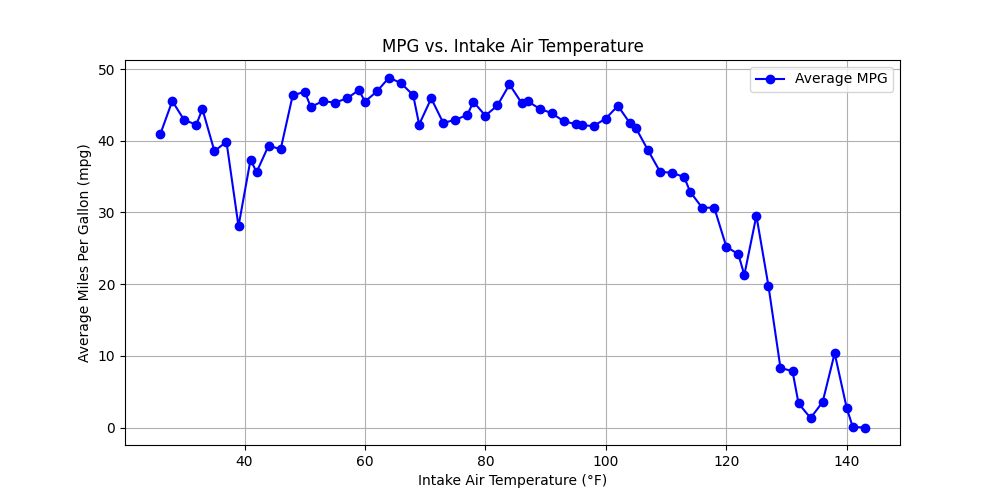
\includegraphics[width=0.4\textwidth]{figures/intake_air_temp_mpg.png}
    \caption{Intake Air Temperature (\textdegree F) vs MPG}
    \label{fig:intakeairtempmpg}
\end{figure}

Related to the temperature of the air coming in is the amount coming in. 
This is determined by the position of the throttle valve. In our case, two 
other factors come into play for the volumetric efficiency of the engine 
for a given throttle position that are a part of Honda's Variable Valve 
Timing and Lift Electronic Control system (VTEC). The iteration of the 
system used in the R18A1 engine of the test vehicle includes two methods 
to additionally control the volume and speed of air entering the engine: 
an additional set of camshaft lobes with lower lift and different 
duration, and valves to change the length of the runners in the intake 
plenum \cite{Bandgar2024}. 

The additional set of camshaft lobes reduces the lift of the intake valves 
and reduces the time they are left open. Furthermore, they are set forward 
of the regular camshaft lobes such that the effective length of the 
engine's intake stroke is reduced. This somewhat mimics the Atkinson cycle 
by making the intake stroke slightly shorter than the power (expansion) 
stroke. The change in effective stroke length has the added benefit of 
improving volumetric efficiency when combined with the ability to further 
open the throttle valve while cruising under light engine loads between 
1,000 and 3,000 RPM, which reduces pumping losses.

At higher RPMs, valves within the intake plenum open to reduce their 
effective length. This has the effect of improving power at the expense 
of fuel economy. Consequently, our dataset contains less of this data, 
along with the fact that this happens at approximately 4500 RPM.

These factors combine for a spike in fuel economy from the throttle 
position most common for coasting with Deceleration Fuel Cutoff (DFCO) 
that sharply tapers off for cruising and acceleration throttle positions 
as shown in Figure \ref{fig:throttlevsmpg}. 

% throttle_vs_mpg.png figure
\begin{figure}[htbp]
    \centering
    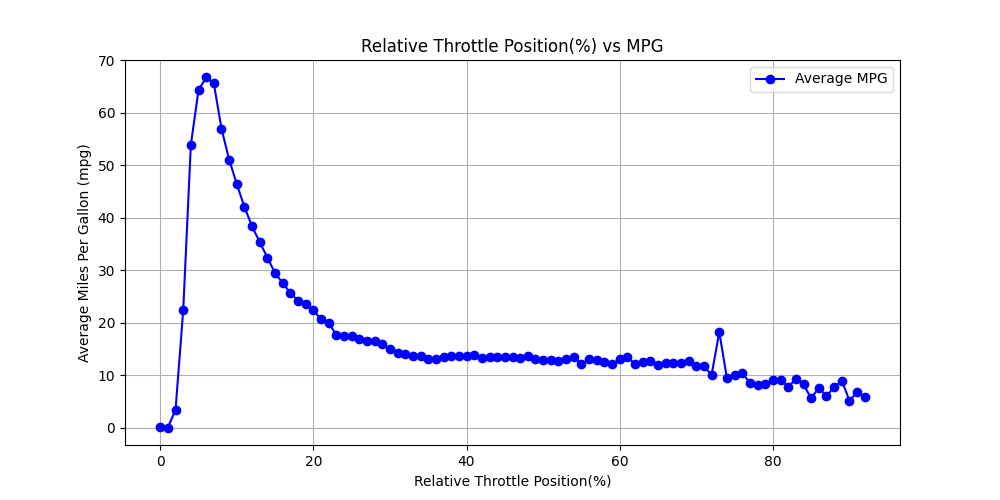
\includegraphics[width=0.4\textwidth]{figures/throttle_vs_mpg.png}
    \caption{Plot of throttle vs MPG}
    \label{fig:throttlevsmpg}
\end{figure}

\subsection*{Extravehicular Factors}

Weather, specifically temperature, was an additional chosen factor as it 
directly correlates with the intake air temperature and air density. 
This directly effects the amount of fuel delivered to the engine as the
ECU attempts to maintain a stochiometric air-fuel ratio. It 
also changes less than the intake air temperature in traffic or other 
conditions where the vehicle is stopped. Finally, seasonal differences in 
fuel blends are dependent on cooler or warmer weather and can be accounted 
for along with the temperature.

Grade was the final factor added as it directly relates to the torque 
required to maintain a given speed (Figure \ref{fig:gradevsmpg}). Going up 
a hill increases this requirement, and going downhill reduces this 
requirement. This is not as important for the fuel economy result, but it 
is important for prediction along the route. We want to predict the fuel 
required to go up a hill, and how much (if any) it will take to go down it. 

\begin{figure}[htbp]
    \centering
    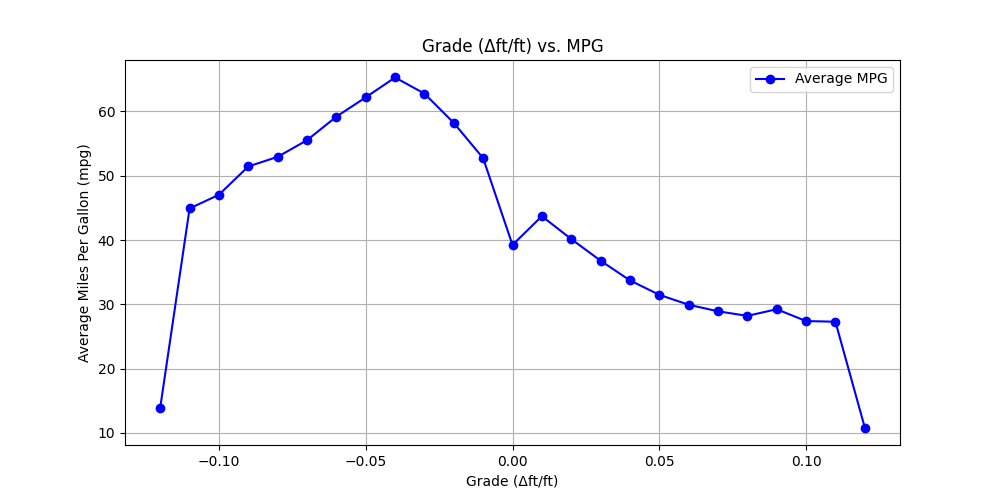
\includegraphics[width=0.4\textwidth]{figures/grade_vs_mpg.png}
    \caption{Plot of Grade vs MPG}
    \label{fig:gradevsmpg}
\end{figure}

\section*{Relation of Variables}

Many of the chosen variables are mathematically related to the fuel 
consumption of the engine by the following equation, where 
$V_{\mathrm{engine}}$ is the volume of the engine in Liters, $N$ is the 
RPM, $\dot{m}_{\mathrm{air}}$ is the air mass flow rate in kg/min, $14.7$ 
is the stochiometric ratio (:1) for a gasoline-air mixture, and $0.74$ is 
the density of gasoline in kg/L.

\[
\text{Fuel volume per minute (L/min)} = \cfrac{\frac{V_{\mathrm{engine}}}{2} \times N \times \dot{m}_{\mathrm{air}}}{14.7\times 0.74}
\]

For this reason, we have included RPM and intake air temperature as 
variables in our model. Related to this is brake-specific fuel consumption 
with the following formula, where $P_{\mathrm{brake}}$ is the brake power 
output of the engine in kilowatts (kW), $\dot{m}_{\mathrm{fuel}}$ is the 
flow rate of fuel in g/h.

\[
\mathrm{BSFC} = \cfrac{\dot{m}_{\mathrm{fuel}}}{P_{\mathrm{brake}}}
\]

Brake power is defined as follows, where $T$ is the torque in Newton-meters 
(Nm) and $9550$ is a constant for unit conversion.

\[
P_{\mathrm{brake}} = \cfrac{T \times N}{9550}
\]

Combining the aerodynamic drag equation, the force of rolling resistance, 
and the grade resistance force; T (the torque required to maintain a given 
speed) is defined as follows, where $C_d$ is the 
drag coefficient, $A$ is the frontal area of the vehicle ($m^2$), $\rho$ 
is the air density in kg/m\textsuperscript{3}, $v$ is the vehicle speed 
in m/s, $C_{rr}$ is the coefficient of rolling resistance of the vehicle, 
$m$ is the mass of the vehicle in kg, $g$ is gravitational acceleration 
($\approx 9.81 \mathrm{m}/\mathrm{s}^2$), Grade is the slope of the road, 
and $R$ is the radius of the tire in(m).

\[
T = (\frac{1}{2}C_d\times A \times \rho \times v^2 + C_{rr} \times m \times g + m \times g \times \frac{\text{Grade (\%)}}{100})\times R
\]

For this reason, altitude, temperature, and intake air temperature have 
been included. 

\cite{hegde2021real} Continue this into time-dependent data by defining a
parametric driver model using speed, acceleration, and driver-dependent
variables to predict driver behavior. Integration of such a model would
enable the predictive usage of our proposed model, along with more 
simplistic approaches to derive things such as RPM from speed and 
estimated gear as in \cite{rykala2023modeling}

\subsection*{Variables Summary}

These variables and equations, however, do not account for road conditions 
or the driver. Hence, there is a need for a more robust, statistical 
approach capable of accounting for the habitual patterns of a human driver.

\section*{K-Fold Cross-Validation}

From our cleaned data, four primary variants were created to test the model 
under different feature conditions. These included a baseline dataset 
without weather data, one with added temperature information, another with 
smoothed inputs, and a final version that also incorporated grade. Each of 
these dataset variations enabled us to examine the specific contributions 
of external environmental conditions and road characteristics to fuel 
delivery prediction.

Model training was conducted using a custom-built recurrent neural network 
architecture, FuelMPGRNN, implemented in PyTorch. The network was designed 
to process sequential input data and predict either a single output 
(instantaneous fuel usage) or a pair of values (instantaneous MPG and 
instantaneous fuel usage). Input sequences consisted of ten consecutive 
timesteps, with each timestep including eight to ten sensor-derived 
features depending on the dataset variant. The model architecture featured 
multiple hidden layers, with key hyperparameters such as hidden state size 
and number of recurrent layers varied across experiments. The training 
process used an 80/20 train-validation split, the Mean Squared Error 
(MSE) loss function, and the Adam optimizer. Models were trained over 100 
epochs and leveraged NVIDIA's CUDA GPU acceleration on an NVIDIA Tesla P40. 
As the models tested were small, they usually shared time with a larger 
model on this GPU.

Evaluation was performed using standard regression metrics, including Root 
Mean Squared Error (RMSE), Mean Absolute Error (MAE), and the coefficient 
of determination (R²). To visualize the model's performance, scatter plots 
comparing predicted and actual values were generated for both fuel 
consumption and trip efficiency. Additionally, a separate set of 
experiments was conducted to compare the performance of models with 
different hyperparameter configurations. This was done using a consistent 
evaluation dataset and measuring the same performance metrics, allowing 
for a fair assessment of the impact of architectural choices such as 
hidden layer size.

Through this experimental setup, we aimed to isolate the effects of each 
feature type and modeling decision, enabling a deeper understanding of how 
telemetry and contextual data can improve predictive models for vehicle 
fuel efficiency.

\section*{Results}

\subsection*{Statistical Models}

\subsection{Linear models}

We present the results of linear regression models that use different 
combinations of vehicle and environmental features. Those models rely on 
the averaged relationships between the input features and the output 
variable. The performance of each model is evaluated using the coefficient 
of determination ($R^2$) and Mean Squared Error (MSE). While these models 
can be good at capturing general trends in data, they remain challenged by 
more complex conditions, and their performance declines when extrapolated 
beyond their training distribution.

To improve the models' ability to capture the upward trend in fuel 
efficiency at lower speeds, we used the square root of speed instead of 
raw speed. This approach allows the models to fit the data up to around 
60 MPH more accurately, which represents the majority of the driving data 
we have. Beyond 60 MPH, the performance of the models declines because the 
variability in MPG increases, and more outliers are detected.

The simplest linear regression model we have only uses the square root of 
speed as a predictor. It was able to achieve a $R^2$ score of 0.6683 and a 
MSE of 93.7981, and the coefficient for sqrt(Speed) in this model is 6.31 
with an intercept of 4.33. This shows that using sqrt(speed) as the only 
feature yields a strong prediction of MPG.

When we added the RPM feature alongside sqrt(speed), the prediction 
performance saw no improvement. The linear regression model in this case 
was able to achieve a $R^2$ score of 0.6672 and a MSE of 94.1096, and the 
coefficients are 6.84 for sqrt(Speed) and -0.0022 for RPM, with an 
intercept of 4.71. This shows that adding RPM to the feature set does not 
improve the performance of the model.

However, when we added the weather data as a feature alongside sqrt(speed), 
the prediction performance saw a noticeable improvement. The linear 
regression model in this case was able to achieve a $R^2$ score of 0.6864 
and a MSE of 88.6874, and the coefficients in this model are 7.29 for 
sqrt(Speed) and -1.25 for the weather feature, with an intercept of 20.29. 
This shows that adding environmental factors to the feature set can 
provide useful context for predicting fuel efficiency, making this 
combination the most effective among the linear models we evaluated.

Table \ref{tab:linear_models_comparison_table} summarizes the results of the 
three models for direct comparison.

\begin{table}
    \centering
    \caption{Comparison of Linear Regression Models}
    \resizebox{\linewidth}{!}{%
    \begin{tabular}{|l|l|c|c|c|}
    \hline
    \textbf{Model} & \textbf{Coefficients} & \textbf{Intercept} & \textbf{$R^2$ Score} & \textbf{MSE} \\
    \hline
    \texttt{$\sqrt{\mathrm{Speed}}$ only} & 6.31 & 4.33 & 0.6683 & 93.7981 \\
    \hline
    \texttt{$\sqrt{\mathrm{Speed}}$ + RPM} & 6.84 (Speed), -0.0022 (RPM) & 4.71 & 0.6672 & 94.1096 \\
    \hline
    \texttt{$\sqrt{\mathrm{Speed}}$ + Weather} & 7.29 (Speed), -1.25 (Weather) & 20.29 & 0.6864 & 88.6874 \\
    \hline
    \end{tabular}
    }
    \label{tab:linear_models_comparison_table}
\end{table}

To provide more insight into the performance of the linear regression 
models, we provide the visualizations for each model. Figure 
\ref{fig:weatherspeedvsmpg} shows  predicted versus actual MPG using 
$\sqrt{\mathrm{Speed}}$ and weather data. Figure \ref{fig:rpmspeedvsmpg}
shows predicted versus actual MPG using $\sqrt{\mathrm{Speed}}$ and RPM 
model. Figure \ref{fig:speedvsmpglinear} shows predicted versus actual MPG 
using $\sqrt{\mathrm{Speed}}$ only. As shown in the visualizations, the 
models' predictions track the true MPG values closely up to around 60 MPH. 
After 60 MPH, the prediction accuracy declines due to increasing 
variability in MPG and the presence of more outliers.

% sqrt_speed_weather_vs_mpg_multiregression_model.png figure
\begin{figure}[htbp]
    \centering
    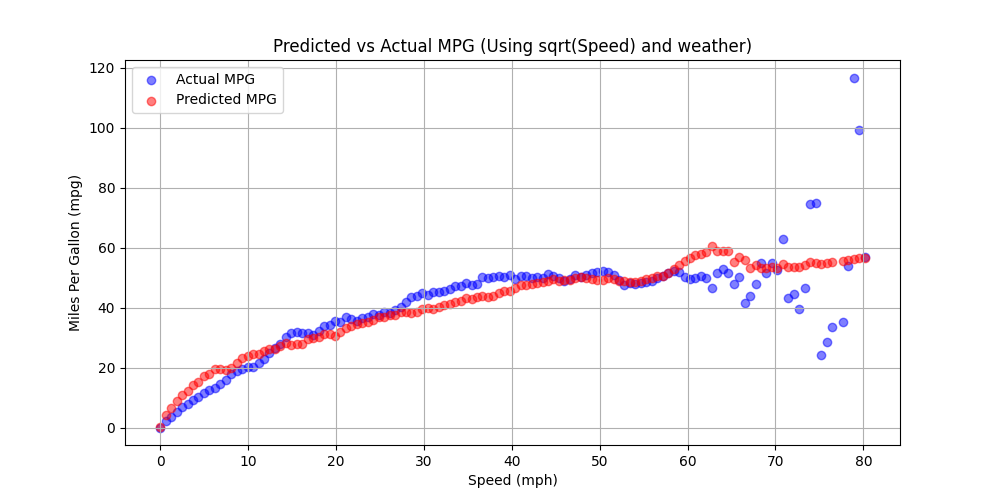
\includegraphics[width=0.4\textwidth]{figures/sqrt_speed_weather_vs_mpg_multiregression_model.png}
    \caption{Plot of MPG predictions of a linear model using speed and weather data.}
    \label{fig:weatherspeedvsmpg}
\end{figure}

% sqrt_speed_rpm_vs_mpg_multiregression_model.png
\begin{figure}[htbp]
    \centering
    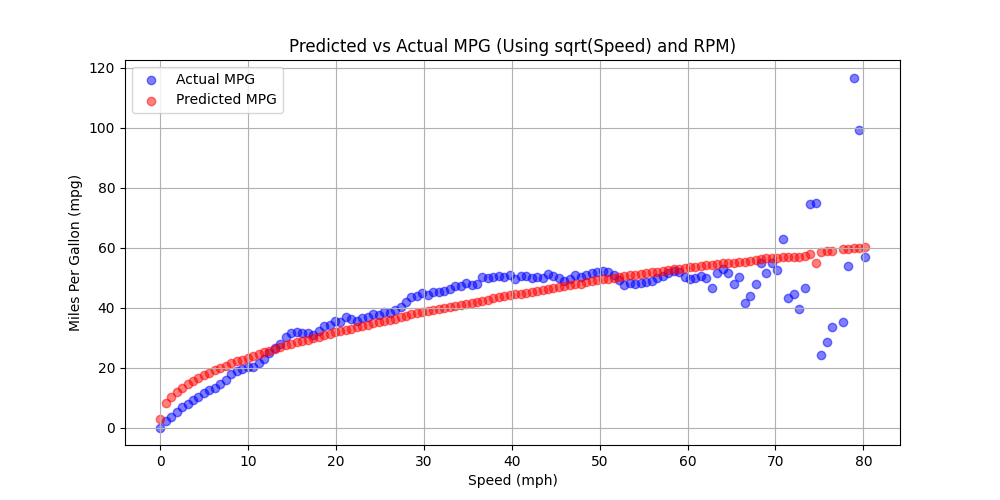
\includegraphics[width=0.4\textwidth]{figures/sqrt_speed_rpm_vs_mpg_multiregression_model.png}
    \caption{Plot of MPG predictions of a linear model using speed and RPM data.}
    \label{fig:rpmspeedvsmpg}
\end{figure}

% speed_vs_mpg_linear_model.png
\begin{figure}[htbp]
    \centering
    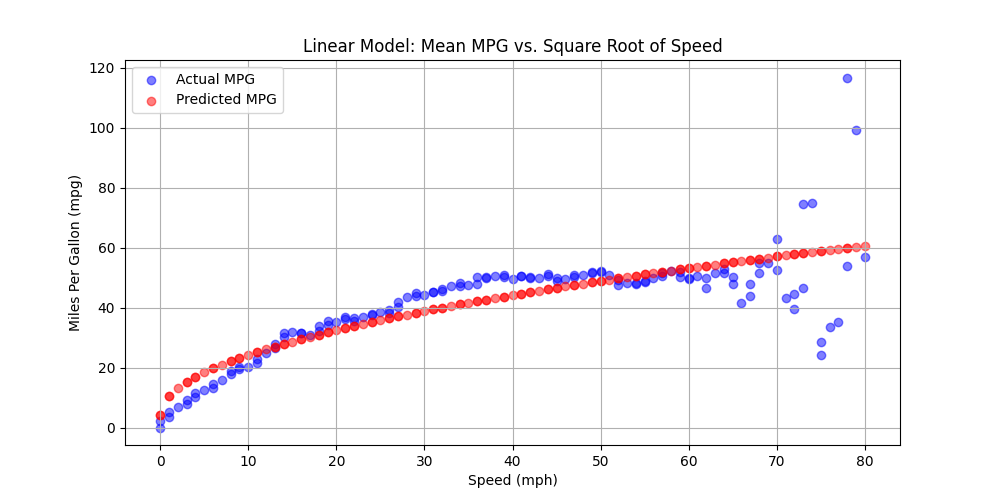
\includegraphics[width=0.4\textwidth]{figures/speed_vs_mpg_linear_model.png}
    \caption{Plot of MPG predictions of a linear model using speed data.}
    \label{fig:speedvsmpglinear}
\end{figure}


\subsection*{LSTM RNN}

\subsubsection*{K-Fold Cross-Validation}

K-fold cross validation was evaluated both on the information extracted 
from the original dataset and the dataset augmented using calculated and 
imported metrics.

An 8-parameter k-fold cross-validation serves as the baseline from which 
other iterations of the algorithm can be evaluated. The parameters used to 
generate this validation were altitude, bearing, air-fuel ratio, engine 
load, engine RPM, intake air temperature, relative throttle position, and 
speed.

\begin{table}[]
    \centering
    \small
    \begin{tabular}{|l|l|l|l|}
        \hline
        \textbf{Layer Num} & \textbf{Hidden Size} & \textbf{$R^{2}$} & \textbf{MAE} \\
        \hline
        2                  & 32                   & 0.4836      & 0.0102       \\
        4                  & 128                  & 0.4662      & 0.0092       \\
        \hline
    \end{tabular}
    \caption{Best-performing models for 8-parameter cross validation.}
    \label{tab:tb1}
\end{table}

The model for this configuration that had the highest $R^{2}$ score had 2 
layers and a hidden layer size of 32, while the model with the lowest MAE 
had 4 layers and 128 nodes in the hidden layers. Performance for these two 
models was generally very similar.

The 9-parameter k-fold cross validation augmented the base case by 
including the outside temperature at the time of driving, in addition to 
the already-existing parameters.

\begin{table}[]
    \centering
    \small
    \begin{tabular}{|l|l|l|l|}
        \hline
        \textbf{Layer Num} & \textbf{Hidden Size} & \textbf{$R^{2}$} & \textbf{MAE} \\
        \hline
        2              	& 64               	& 0.4798  	& 0.0097   	\\
        4              	& 128              	& 0.4542  	& 0.0091 	\\
        \hline
    \end{tabular}
    \caption{Best performing models for 9-parameter cross-validation.}
    \label{tab:tb2}
\end{table}

The better-performing model architectures for the 9-parameter data follow 
a similar pattern to the 8-parameter data. However, in order to achieve an 
optimal $R^{2}$ score, the size of the hidden layer had to be doubled from 
32 to 64. The most likely cause of this is the increased complexity from 
the additional parameter.

The slope grade for a particular interval of the road was added to the 
9-parameter dataset to see how that increased model performance. This 
value was calculated from the change in altitude for a specific interval 
at a given speed.

\begin{table}[]
    \centering
    \small
    \begin{tabular}{|l|l|l|l|}
        \hline
        \textbf{Layer Num} & \textbf{Hidden Size} & \textbf{$R^{2}$} & \textbf{MAE} \\
        \hline
        2              	& 256              	& 0.6227  	& 0.0116   	\\
        4              	& 128              	& 0.5057  	& 0.0102 	\\
        \hline 
    \end{tabular}
    \caption{Best performing models for 9-parameter cross-validation w/ slope grade.}
    \label{tab:tb3}
\end{table}

The best-performing $R^{2}$ results for this permutation of data continue 
to follow the pattern set by the previous model: a drastic increase in 
hidden layer size was required to attain optimal results. Interestingly, 
the increase resulted in a marked improvement in $R^{2}$ compared to the 
difference between the 8-parameter and 9-parameter datasets.

Another interesting thing to note is that the 4-layer 128-hidden-layer-size 
continues to provide the best MAE out of all sizes evaluated. Even though 
both models improved on $R^{2}$, the MAE increased, most likely due to the 
added complexity of the grade parameter.

Because the amount of fuel used is inversely correlated with the fuel 
economy, theoretically one can be calculated if the other is accurately 
predicted by the model. The dataset augmented with weather data and slope 
grade was used to predict only fuel use, and from that, fuel economy was 
calculated.

This configuration resulted in one of the best performing models in all of 
the entire results. The model had 6 layers and a hidden layer size of 64, 
and it was able to obtain both the highest $R^{2}$ score and lowest MAE 
value at 0.8794 and 0.0013, respectively.

The final modification to the dataset tested was removal of the bearing 
parameter. Again, only the fuel use was predicted, and weather data and 
slope grade were included.

\begin{table}[]
    \centering
    \small
    \begin{tabular}{|l|l|l|l|}
        \hline
        \textbf{Layer Num} & \textbf{Hidden Size} & \textbf{$R^{2}$} & \textbf{MAE} \\
        \hline
        4              	& 64               	& 0.8234  	& 0.0014   	\\
        6              	& 128              	& 0.8205  	& 0.0014 	\\
        \hline
    \end{tabular}
    \caption{Best performing models for weather and grade, bearing omitted.}
    \label{tab:tb4}
\end{table}

The overall performance of the models in this situation was reduced by a 
noticeable amount. In both models, $R^{2}$ was reduced by about 0.05. MAE 
saw a drop that can be considered inconsequential; approximately 0.0001.

\subsubsection*{Brake-Specific Fuel Consumption}

An alternative model architecture was proposed and implemented in an effort 
to broaden understanding of the target problem. The model implemented a 
RNN with long short-term memory (LSTM) and linearization layers.

The brake-specific fuel consumption (BSFC) was used to estimate fuel 
consumption using the torque, load, and RPM of the engine. These values 
were included as part of an alternative dataset, the POLIDriving dataset.

Training on this data, the model attempted to predict a flow rate in liters 
per hour, which was compared to the value from the BSFC calculation. Over 
the course of 100 epochs, the model was able to successfully learn the fuel 
usage, and it had a total loss at the end of training of 3.0846 
(Figure \ref{fig:lossrnn}).

\begin{figure}[h!]
    \centering
    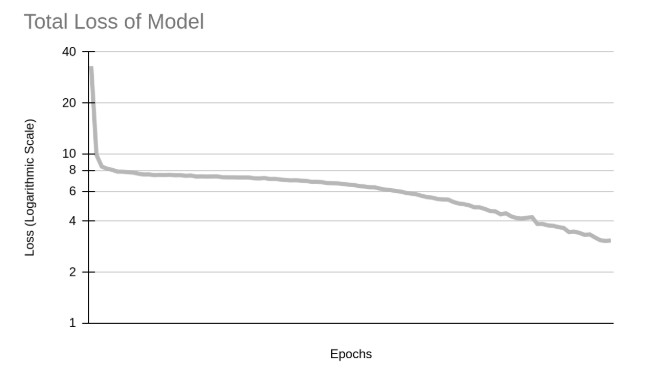
\includegraphics[width=0.4\textwidth]{figures/loss.jpg}
    \caption{Loss of the RNN on the POLIDriving dataset}
    \label{fig:lossrnn}
\end{figure}

When compared against the original data, the model was able to closely 
match the true value (Figure \ref{fig:predictionrnn}).\\

% rnn_predictions.png
\begin{figure}[h!]
    \centering
    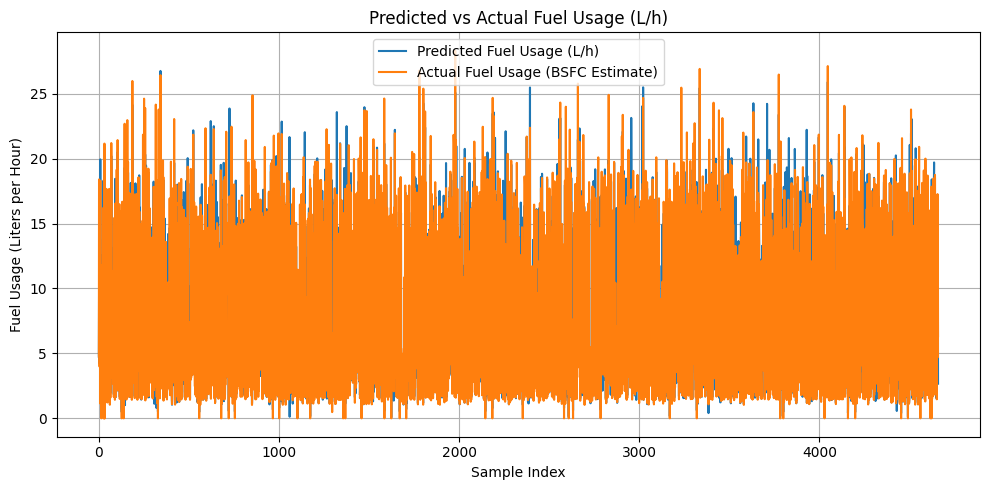
\includegraphics[width=0.38\textwidth]{figures/rnn_predictions.png}
    \caption{Predictions of the RNN on the POLIDriving dataset}
    \label{fig:predictionrnn}
\end{figure}

\subsubsection*{Final Model}

A final model was trained using what was considered to be the best 
combination of parameters and hyperparameters. The number of layers chosen 
was 6, and the size of the hidden layers was 64.

The dataset chosen was the final one evaluated, where bearing was 
included. Again, the amount of fuel used was predicted and fuel economy 
calculated from that.

The overall metrics for the model are as follows:

\begin{table}[h!]
    \centering
    \small
    \begin{tabular}{|l|l|}
        \hline
        Metric & Value \\
        \hline
        MAE          	& 0.00097	\\
        MSE          	& 0.000003   \\
        R2 Score     	& 0.954  	\\
        SAE          	& 552.4384   \\
        SSE          	& 1.8007 \\
        \hline
    \end{tabular}
    \caption{Performance metrics of final model after training.}
    \label{tab:my-table}
\end{table}

Comparing the predicted fuel consumption total against the actual total 
resulted in a total error of 2.8742\%. These results further reinforce the 
conclusion that our proposed ``optimal'' model is well-suited with the 
chosen features extracted from the dataset.

Finally, an analysis of the computational load of this final model was 
carried out using the \verb|fvcore| Python module. On a batch size of 1, 
the model required approximately 1.8 MFLOPS. Modern graphics cards are 
capable of handling orders of magnitude more data, and even the Intel 
i386 microprocessor can run a similar amount of calculations 
(https://www.jcmit.net/cpu-performance.htm).

\section{Conclusion}

This investigation has sought to evaluate how various factors, both 
internal and external to a motor vehicle, affect its fuel economy. This 
was accomplished through the creation of a base dataset using vehicle 
statistics gathered from the OBD-II interface.

This data was augmented through the collection of external features, 
such as weather data from a freely-available API, and calculation of 
variables not collectable by the used interface, such as road grade.

Various configurations of RNNs were constructed and allowed to train on 
parameters from the input data. Hyperparameters were adjusted several 
times in order to evaluate the performance of different architectures 
and how they adapt to the data. Finally, the best of both the models and 
dataset permutations were paired together to understand how a best case 
scenario would perform.

\section{Limitations}
Both the data and methodology face limitations in their scope and 
applicability. The data collected from the OBD-II sensor is only 
applicable to the model car, and the trained neural network may not 
accurately be able to predict fuel economy on different vehicles. This 
would be even worse in situations where gasoline is not the only method 
of propulsion (hybrids and electric vehicles) or fuels with different
combustion rates (diesel, biodiesel, jet fuel) must be factored in.

Additionally, the style of driving the operator of the vehicle has 
resulted in a significant impact on fuel usage. There is no 
quantification of how the driver of the model vehicle drove, and this 
investigation would most likely have enough substance to be its own paper. 
It is with some hope that the RNN was able to ``learn'' our test driver's 
style by proxy of other metrics, such as RPM and vehicle speed.

One of our desired use cases for this model is as an in-vehicle assistant 
capable of learning the vehicle's average fuel consumption and driver's 
driving style well enough to estimate the remaining mileage a car has 
before running out of fuel. Unfortunately, to test the practicality of 
this system with our model would require specialized IoT or embedded 
hardware we do not have access to. We can only estimate this by proxy of 
the results gathered from the \verb|fvcore| evaluation.

\bibliographystyle{aaai} 
\bibliography{references_final.bib}

\end{document}